% Edicion abreviada de Beamer original slides/final.tex (PR #90).
% Seleccion: 1, 2, 3, 7, 8, 9, 10, 15, 17, 19, 20, 24, 25, 26, 28, 30, 33, 34 de los 43 frames, sin alterar contenido de figuras y ecuaciones.
% 23 minutos de discurso y 2 de transiciones; no reemplaza el Beamer completo.
% Presentacion Beamer original: revision oral postplazo, 28/11/2026.
% Conserva las figuras y las IRF del proyecto; no certifica equilibrio completo.
\documentclass[aspectratio=169,11pt]{beamer}
\usepackage[utf8]{inputenc}
\usepackage[T1]{fontenc}
\usepackage[spanish,es-nodecimaldot]{babel}
\usepackage{lmodern,amsmath,amssymb,booktabs,graphicx}
\usepackage{tikz}
\usetikzlibrary{arrows.meta,calc,positioning,babel}
\usetheme{default}
\usecolortheme{seahorse}
\setbeamertemplate{navigation symbols}{}
\setbeamertemplate{footline}[frame number]
\setbeamersize{text margin left=0.85cm,text margin right=0.85cm}
\definecolor{deepnavy}{RGB}{24,47,74}
\setbeamercolor{structure}{fg=deepnavy}
\setbeamercolor{frametitle}{fg=deepnavy,bg=white}
\setbeamerfont{frametitle}{size=\large}
\title{Política monetaria, liquidez bancaria\\y asignación de capital}
\subtitle{Exposición de 25 minutos: mecanismos, evidencia y límites}
\author{Alejandro Ventura}
\date{Edición oral abreviada: 28 de noviembre de 2026}
\begin{document}

% Source Beamer original frame 1
\begin{frame}[plain]\titlepage
\centering\footnotesize
\url{https://github.com/alejandroventuraventurameza-tech/ai-project}
\end{frame}

% Source Beamer original frame 2
\begin{frame}{Pregunta y resultado que sometemos a revisión}
¿Cuándo una intervención monetaria facilita capital a empresas productivas?
\medskip
\[
\text{Banco central}\longrightarrow\text{interbancario}\longrightarrow
\text{bancos comerciales}\longrightarrow\text{empresas}.
\]
\begin{itemize}
\item El experimento interno conserva dos ramas del sistema reducido.
\item En ambas baja la tasa de crédito y aumenta el crédito de H.
\item La pérdida asignativa cae en S y sube en B: el signo es condicional, y la mejora no se infiere solo de $A_H>A_L$.
\end{itemize}
\medskip
\textbf{Alcance:} parámetros ilustrativos, pagos finitos e IRF locales;
la correspondencia completa con equilibrio óptimo sigue pendiente.
\end{frame}

% Source Beamer original frame 3
\begin{frame}{Convenciones: agentes, empresas y ramas}
\small
\begin{itemize}
\item $W$: hogar trabajador; $E$: empresario; $i\in\{H,L\}$: tipo de firma.
\item $H$: productividad tecnológica alta ($A_H>A_L$); $L$: productividad tecnológica baja. La productividad marginal del capital depende también de $k_i$ y $\ell_i$.
\item $j$: banco; el superíndice $B$ en $l^B,m^B,s^B$ significa \emph{bancario}, no la rama B.
\item $S,B$: ramas \emph{del sistema reducido}, no tipos de hogar o empresa.
\item $R^R$: remuneración de reservas; $R^W$: facilidad; $R^F$: interbancaria; $R^L$: préstamo; $R^D$: depósito. Todas son tasas brutas.
\item $\rho$: coeficiente de encaje; $\Delta=R^W-R^R$: amplitud del corredor.
\end{itemize}
\medskip
\textbf{Advertencia:} $H_{it}$ es el valor pignorable por unidad de capital, no el tipo de empresa H; el contexto y los índices los distinguen.
\end{frame}

% Source Beamer original frame 7
\begin{frame}{Empresa: qué maximiza y qué la limita}
\[
V_i(N,\mathcal S)=\max_{c,k',b,a}\{u_E(c)+\beta_E\mathbb E V_i(N',\mathcal S')\}.
\]
\[
c+q_t k'+a=N+b,\qquad
R^L_t b\leq\theta_i(1-\delta)\inf_{s'}\{\Pi_{t+1}q_{t+1}\}\,k'.
\]
\begin{itemize}
\item Caja: consumo, inversión y ahorro se financian con patrimonio y préstamo.
\item Garantía: el repago nominal debe estar cubierto en cada estado admisible.
\item Una tasa menor amplía capacidad financiable a garantía dada, pero precios,
patrimonio y demandas también reaccionan.
\item $A_H>A_L$ no garantiza por sí solo una mejora asignativa.
\end{itemize}
\end{frame}

% Source Beamer original frame 8
\begin{frame}{Bancos comerciales y mercado interbancario}
\[
l^B+m^B=d^D+x,\quad x=e-d^B>0,\quad
 d^D\leq\kappa_Dx,\quad l^B\leq\kappa_Lx.
\]
El banco maximiza dividendos y valor futuro descontado, con salida y solvencia
por estado. Después del pago, su exceso de reservas sobre encaje es
\[
s^B=m^B-\rho d^D+(R^D/R^R-\rho)\omega d^D.
\]
\begin{itemize}
\item El interbancario redistribuye reservas entre bancos con déficit y excedente.
\item La facilidad del banco central cubre parte del déficit no negociado.
\item Crédito a empresas y crédito entre bancos son contratos diferentes.
\end{itemize}
Los instrumentos son remuneración y cantidad de reservas, encaje y corredor.
Aquí variamos solo la innovación de remuneración.
\end{frame}

% Source Beamer original frame 9
\begin{frame}{Mercado OTC y formación endógena de tasas}
\small
\[
S^-=\sum_j u_j\mathbb E_\omega(-s_j^B)^+,\quad
S^+=\sum_j u_j\mathbb E_\omega(s_j^B)^+,\quad
\vartheta=S^-/S^+.
\]
La negociación y el corredor determinan la tasa interbancaria; $R^W$ es el techo y $R^R$ el piso en el cierre adoptado:
\[
R^F_t=R^R_t+(R^W_t-R^R_t)v(\vartheta_t).
\]
Las condiciones interiores de precios bancarios auditadas implican
\[
R^L_t=R^R_t+\bar\chi_t,
\]
\[
R^D_t=R^R_t+(1-\rho)\bar\chi_t-
\left(\frac{R^D_t}{R^R_t}-\rho\right)
\frac{\zeta(\chi^-_t-\chi^+_t)}{2}.
\]
\footnotesize
El shock cambia $R^R$; la respuesta de $R^F,R^L,R^D$
depende del ajuste simultáneo de matching, pagos y carteras.
\end{frame}

% Source Beamer original frame 10
\begin{frame}{Corredor: nivel, amplitud e incentivos}
\small
\[
R^W_t=R^R_t+\Delta_t,\qquad
R^F_t=R^R_t+\Delta_t\,v(\vartheta_t),\qquad 0\leq v(\vartheta_t)\leq 1.
\]
\begin{itemize}
\item \textbf{Subir $R^W$ manteniendo $R^R$:} ensancha el corredor por arriba; no es un desplazamiento paralelo.
\item \textbf{Bajar $\Delta$ manteniendo $R^R$:} estrecha el corredor; cambia el costo máximo de obtener liquidez, no necesariamente la remuneración de excedentes.
\item \textbf{Mover $R^R$ y $R^W$ en igual magnitud:} desplaza el corredor conservando su amplitud.
\item Un banco excedentario compara colocar reservas remuneradas con prestarlas en OTC, considerando probabilidad de encuentro y condiciones de negociación.
\end{itemize}
\textbf{Importante:} la respuesta de $R^D$ y $R^L$ es endógena a balances, depósitos, márgenes de cartera y liquidez; no se deduce únicamente del dibujo del corredor.
\end{frame}

% Source Beamer original frame 15
\begin{frame}{Productividad marginal, colateral y reasignación}
\small
Para $F_i=A_i k_i^\alpha \ell_i^\beta$, con $\alpha,\beta>0$:
\[
MPK_i=\alpha A_i k_i^{\alpha-1}\ell_i^\beta,\qquad
MPL_i=\beta A_i k_i^\alpha\ell_i^{\beta-1}.
\]
\begin{itemize}
\item $A_H>A_L$ \emph{no} implica $MPK_H>MPK_L$: importan también las dotaciones de capital y trabajo.
\item Una reasignación marginal de capital a trabajo dado aumenta producción solo si el $MPK$ del receptor excede el del cedente, con precios y restricciones pertinentes.
\item Si el colateral está activo, $R^L b_i=H_{it}k'_i$; bajar $R^L$ aumenta \emph{parcialmente} la capacidad financiable, no necesariamente reduce el multiplicador $\mu_i$.
\item Subir $\theta_i$ expande el valor pignorable $H_{it}$ manteniendo los demás factores constantes. $\theta_i$ es parámetro contractual, no un instrumento monetario.
\end{itemize}
\end{frame}

% Source Beamer original frame 17
\begin{frame}{Regla monetaria y experimento identificado}
\small
El experimento cambia una sola innovación de la regla de remuneración:
\[
\Delta\log R^R_t
=0.5\Delta\log R^R_{t-1}
+0.75\Delta\log\Pi_t+0.0625\Delta\log Y_t+v_t.
\]
\[
v_0=-10^{-5},\quad v_t=0\ (t\geq1),\quad
\rho=0.10\text{ fijo.}
\]
La tasa efectiva responde endógenamente a inflación y producto, por lo
que su movimiento total no es igual al shock de regla.
\medskip
\begin{itemize}
\item Aproximadamente $-0.1$ pb como innovación inicial; sin shocks futuros.
\item Es un shock a la \emph{remuneración}, no al coeficiente de encaje.
\item Se conservan las mismas posiciones heredadas y las dos ramas S/B.
\end{itemize}
\end{frame}

% Source Beamer original frame 19
\begin{frame}{Sistema reducido, regiones financieras y multiplicidad}
\small
El problema computacional usa 33 logvariables y 33 relaciones
(17 en fecha 0 y 16 en fecha 1):
\[
F_r(Z,\mathbf v)=0,\quad Z\in\mathbb R^{33},\quad r\in\{S,B\}.
\]
Con H restringida, la condición de L se reduce localmente a
\[
0\leq s_{L0}\perp\mathcal M(s_{L0},\mathbf v)\geq0,\qquad
\mathcal M(s,\mathbf v)=\mathbf a^\top\mathbf v+bs
+o(\|(s,\mathbf v)\|).
\]
En la calibración ilustrativa, $a_R\simeq-3.219277533$ y
$b\in(-2.376742673,-2.376742670)$.
\begin{itemize}
\item S: $s_{L0}>0$ y dual de L nulo; B: $s_{L0}=0$ y dual no negativo.
\item Estas son soluciones locales del \emph{sistema reducido}; la
correspondencia con equilibrio competitivo completo no está cerrada.
\end{itemize}
\end{frame}

% Source Beamer original frame 20
\begin{frame}{Derivación: exactamente dos soluciones escalares}
\small
Suponga que $\mathcal M(s,h)$ es $C^1$ cerca de cero,
$\mathcal M(0,0)=0$, $a_R=\partial_h\mathcal M(0,0)<0$
y $b=\partial_s\mathcal M(0,0)<0$.
\[
0\leq s\perp \mathcal M(s,h)\geq0.
\]
Si $h<0$, la función implícita produce una
raíz $s(h)>0$, pues $s'(0)=-a_R/b<0$.
\[
\boxed{\begin{aligned}
B:&\ s=0,\quad \mathcal M(0,h)>0,\\
S:&\ s=s(h)>0,\quad \mathcal M(s(h),h)=0.
\end{aligned}}
\]
\footnotesize
La monotonía decreciente excluye una tercera raíz
positiva cercana; para $h>0$, la condición de signo
impide toda solución complementaria local.
\textbf{Es una proposición del reducido, no de
equilibrio competitivo infinito.}
\end{frame}

% Source Beamer original frame 24
\begin{frame}{Transmisión financiera: las dos respuestas}
\centering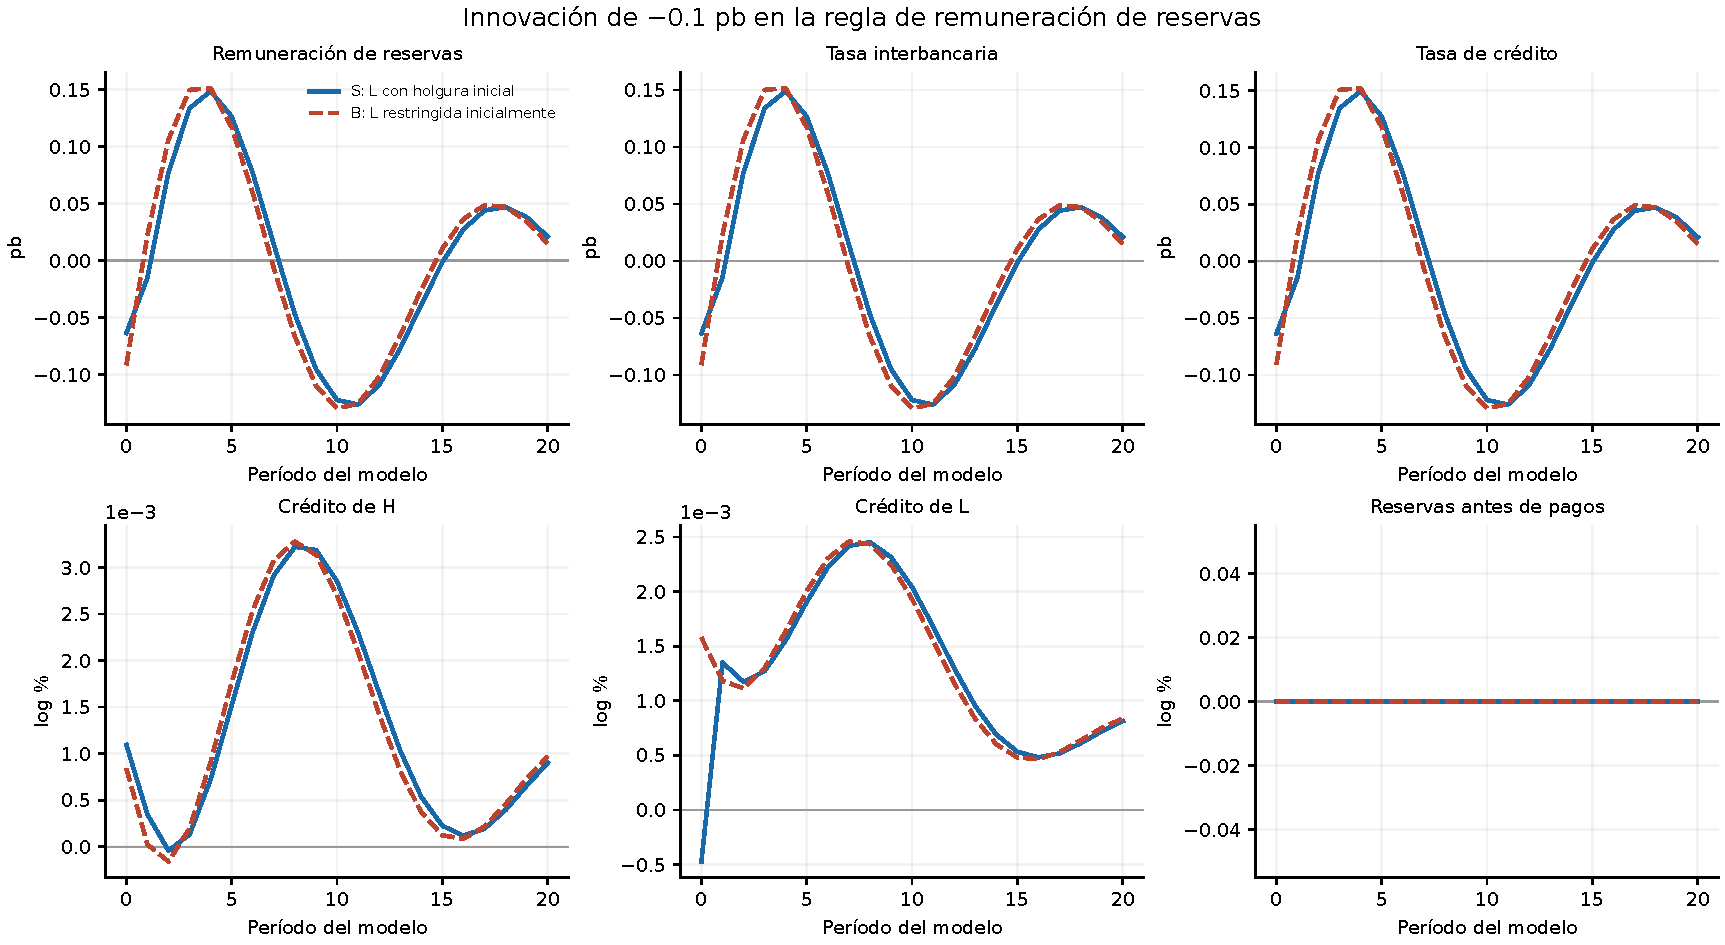
\includegraphics[height=.79\textheight,width=\textwidth,keepaspectratio]{../paper/figures/irf_transmission.pdf}
\end{frame}

% Source Beamer original frame 25
\begin{frame}{Capital, producción y pérdida asignativa}
\centering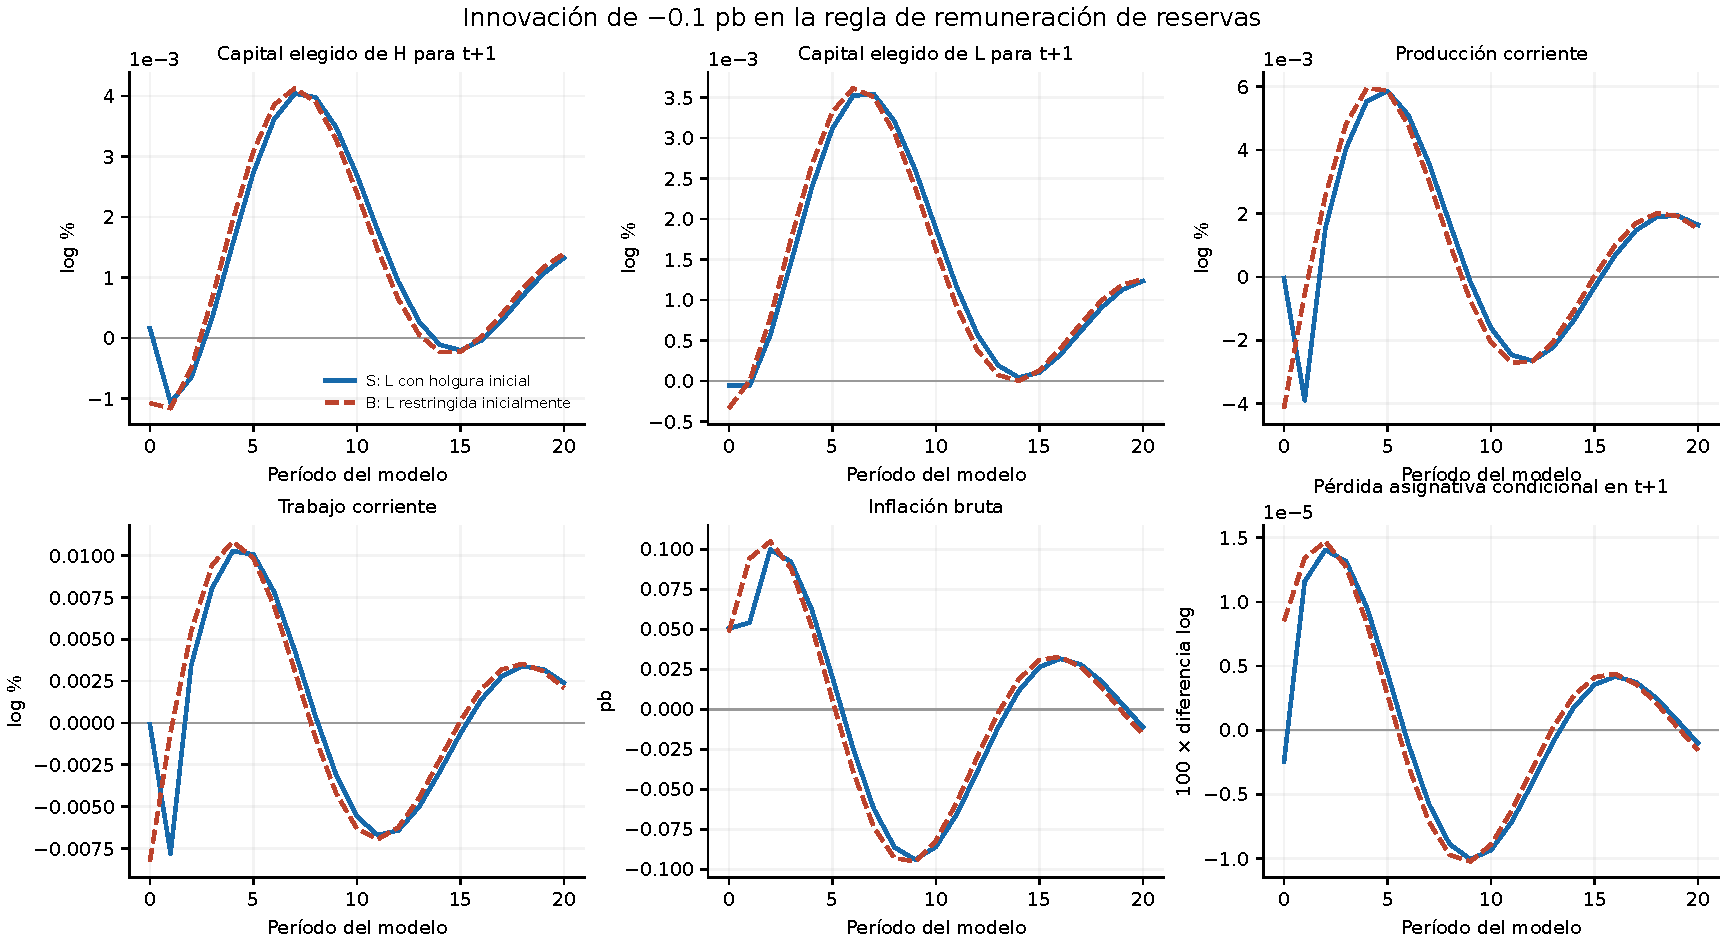
\includegraphics[height=.79\textheight,width=\textwidth,keepaspectratio]{../paper/figures/irf_real_allocation.pdf}
\end{frame}

% Source Beamer original frame 26
\begin{frame}{El mismo crédito puede financiar menos capital}
\footnotesize
Para H con garantía activa, $n_H=N_H-c_H$ y
$p_H^{\mathrm{eff}}=q-H_H/R^L>0$:
\[
100\Delta\log k'_H=100\Delta\log n_H
-100\Delta\log p_H^{\mathrm{eff}},
\]
\[
100\Delta\log b_H=
100\Delta\log H_H+100\Delta\log k'_H-100\Delta\log R^L.
\]
\begin{center}
\resizebox{.96\linewidth}{!}{% Generated by code/irf/render_mechanism_table.py; do not edit numeric cells by hand.
% T=640 nonlinear finite system, branch-specific reference; values are accounting log contributions.
\begin{tabular}{@{}lrr@{}}\toprule
Magnitud de impacto & Rama S & Rama B\\\midrule
Recursos invertibles $100\Delta\log(N_H-c_H)$ & 0.00002735 & -0.00174198\\
Menor precio efectivo $-100\Delta\log(q-H/R^L)$ & 0.00013674 & 0.00066934\\
\textbf{Capital elegido} $100\Delta\log k_{H,t+1}$ & 0.00016409 & -0.00107264\\
\addlinespace[2pt]
Valor pignorable $100\Delta\log H_H$ & 0.00031268 & 0.00102984\\
Menor tasa $-100\Delta\log R^L$ & 0.00061840 & 0.00088344\\
\textbf{Crédito} $100\Delta\log b_H$ & 0.00109517 & 0.00084064\\
\addlinespace[2pt]
Dual normalizado $10^6\Delta\upsilon_H$ & -1.21674 & 23.08136\\
\bottomrule\end{tabular}
}
\end{center}
\vspace{-0.15cm}% evitar desbordamiento vertical observado en el build
\scriptsize
\textbf{Fuente:} \texttt{audit\_financial\_blocks.py} y
\texttt{render\_mechanism\_table.py}, solución no lineal finita $T=640$.
En B cae el recurso invertible lo suficiente para superar la
reducción del precio efectivo; por eso $k'_H$ cae aunque $b_H$ suba.
Estas contribuciones son identidades en equilibrio conjunto,
no intervenciones causales separadas.
\end{frame}

% Source Beamer original frame 28
\begin{frame}{Qué ocurre al impacto}
\centering\small\begin{tabular}{lrr}\toprule
Respuesta al impacto & S & B\\\midrule
Tasa interbancaria (pb) & -0.06363254 & -0.09117145\\
Tasa de crédito (pb) & -0.06363175 & -0.09090760\\
Producción (log \%) & -0.00003580 & -0.00414255\\
Crédito H (log \%) & 0.00109518 & 0.00084065\\
Crédito L (log \%) & -0.00047390 & 0.00157811\\
Pérdida condicional ($100\Delta\log$) & -0.00000248 & 0.00000852\\
\bottomrule\end{tabular}

\medskip\par\raggedright
La pérdida es $\log(Y^{ef}_{t+1}/Y_{t+1})$ a recursos agregados dados del período
siguiente. No mide bienestar ni identifica una fricción financiera con datos.
\end{frame}

% Source Beamer original frame 30
\begin{frame}{La producción cae inicialmente: resultado que debemos explicar}
El capital instalado es predeterminado y el trabajo cae en ambos tipos.
Para la tecnología del ejercicio, la condición laboral implica al impacto:
\[
\Delta\log\ell_i=2(\Delta\log m-\Delta\log w),\qquad
\Delta\log y_i=\tfrac12\Delta\log\ell_i.
\]
\[
\Delta Y=\Delta C+\Delta\Gamma+\Delta\mathcal R.
\]
\begin{itemize}
\item El reproductor verifica las identidades laborales y de recursos.
\item Crédito más barato no implica mayor producción corriente automáticamente.
\item Estas identidades ubican el ajuste inmediato; la interpretación estructural
completa requiere cerrar optimalidad y equilibrio. No imponemos el signo.
\end{itemize}
\end{frame}

% Source Beamer original frame 33
\begin{frame}{Adenda técnica: alcance de la formalización (28/11)}
\small
\begin{block}{Comprobado en Lean, con condiciones explícitas}
\begin{itemize}
\item Ocho resultados del artículo: validación de la interfaz
\emph{paper-scoped} con el generador oficial y \texttt{check --fast}.
\item Dos filas monetarias SOURCE: derivadas de Fréchet
\emph{condicionadas} a las derivadas de $\log(Y/\bar Y)$.
\item Producto agregado SOURCE: regla exacta de suma ponderada
de las derivadas de las firmas H y L.
\end{itemize}
\end{block}
\begin{alertblock}{No demostrado por esos controles}
La derivabilidad Cobb--Douglas con trabajo endógeno, el Jacobiano
SOURCE completo, su invertibilidad y dos equilibrios competitivos dinámicos.
\end{alertblock}
\footnotesize
Evidencia posterior a la entrega: PR \#83, \#86 y \#88;
la extensión del logaritmo del producto está todavía en revisión.
\end{frame}

% Source Beamer original frame 34
\begin{frame}{Resultado para discusión y siguiente paso}
\textbf{Hallazgo del ejercicio:} la misma innovación puede generar respuestas
asignativas opuestas según la rama, aunque ambas abaraten el crédito.
\medskip
\begin{itemize}
\item Conservar las dos ramas y sus condiciones.
\item Revisar el mecanismo que determina producción y trabajo al impacto.
\item Completar la validación interna antes de estimar o calibrar con datos.
\end{itemize}
\medskip
Reproducción: \texttt{python code/verify.py}.
\par Artículo extenso, tablas automáticas y figuras disponibles para revisión.
\end{frame}
\end{document}
